\documentclass{article}
\usepackage[utf8]{inputenc}
\usepackage[landscape]{geometry}
\usepackage{enumitem}
\usepackage{float} % use H for figure placement
\usepackage{pgfplots}
\usepackage{multicol,multirow}
\usetikzlibrary{arrows}
\usepackage{amsmath,amssymb}
\usepackage{hyperref}
\usepackage[amsthm]{ntheorem}
\usepackage{xcolor}
\usepackage{framed}
\definecolor{shadecolor}{rgb}{0.95,0.95,0.95}
\usepackage{physics}

\newtheorem{theorem}{Theorem}[section]
\newtheorem{prop}{Proposition}
\newtheorem{corollary}{Corollary}
\newtheorem{lemma}{Lemma}
\newtheorem{ex}{Example}
\newtheorem*{remark}{Remark}
\theoremstyle{definition}
\newtheorem{definition}{Definition}[section]

\usepackage [autostyle, english = american]{csquotes}
\MakeOuterQuote{"}
\newcommand{\Section}[1]{\hrule\hrule\section{#1}}
\newcommand{\Def}[2]{
\begin{shaded*}
\begin{definition}{\textit{#1}}\\#2\end{definition}
\end{shaded*}
}
\DeclareMathOperator*{\argmin}{arg\,min}
\DeclareMathOperator*{\argmax}{arg\,max}
\def\R{\mathbb{R}}
\def\C{\mathbb{C}}

\def\conv{\circledast}

\ifthenelse{\lengthtest { \paperwidth = 11in}}
{ \geometry{top=.5in,left=.5in,right=.5in,bottom=.5in} }
{\ifthenelse{ \lengthtest{ \paperwidth = 297mm}}
	{\geometry{top=1cm,left=1cm,right=1cm,bottom=1cm} }
	{\geometry{top=1cm,left=1cm,right=1cm,bottom=1cm} }
}
\pagestyle{empty}
\makeatletter
\renewcommand{\section}{\@startsection{section}{1}{0mm}%
	{-1ex plus -.5ex minus -.2ex}%
	{0.5ex plus .2ex}%x
	{\normalfont\large\bfseries}}
\renewcommand{\subsection}{\@startsection{subsection}{2}{0mm}%
	{-1explus -.5ex minus -.2ex}%
	{0.5ex plus .2ex}%
	{\normalfont\normalsize\bfseries}}
\renewcommand{\subsubsection}{\@startsection{subsubsection}{3}{0mm}%
	{-1ex plus -.5ex minus -.2ex}%
	{1ex plus .2ex}%
	{\normalfont\small\bfseries}}
\makeatother
\setcounter{secnumdepth}{0}
\setlength{\parindent}{0pt}
\setlength{\parskip}{0pt plus 0.5ex}

\title{ENM 521 - MechE Math part 2 - Cheat sheet}
\author{Rebecca Li}
\date{Fall 2019}

\begin{document}
ENM 521


\raggedright
\footnotesize
\begin{multicols}{3}
	\setlength{\premulticols}{1pt}
	\setlength{\postmulticols}{1pt}
	\setlength{\multicolsep}{1pt}
	\setlength{\columnsep}{2pt}
\section{tricks}
Take the derivative
Bound to zero
Do contours around the branch cut (keyhole)
Exponentials are faster than polynomials 

\subsection{Summation/Integration techniques}
$\sum_{j=1}^{n} \sum_{k=1}^{j} f(j,k) = \sum_{k=1}^{n} \sum_{j=k}^{n} f(j,k) $

$\sum_{j=0}^{\infty} \sum_{k=0}^{\infty} f(j,k) = \sum_{n=-\infty}^{\infty} \sum_{k=0}^{\infty} f(n+k,k) $

Change of variables:
$\int_{\phi(a)}^{\phi(b)} f(u)du = \int_{a}^{b} f(\phi(x)) phi'(x)dx$
$\iint_R f(x,y) dA = \iint_S f(g(u,v), h(u,v)) \left|\pdv{(x,y)}{(u,v)}\right| d\bar{A}$

Integration by Parts:
$\int_a^b u dv = uv|_a^b - \int_a^b v du $

Integral in spherical over whole domain:
$x = \rho \sin \phi \cos \theta,\ y = \rho \sin \phi \sin \theta,\ \rho \cos \phi $
$\rho \in [0, \infty ], \theta \in [0, \pi], \phi \in [0, 2\pi]$
$dV = \rho^2 \sin \phi d\rho d\theta d\phi$

Bounding:
$|e^{e^{i\theta/2} + tRe^{i\theta}}| \leq e^{\cos(\theta/2) + Rt\cos\theta}$
\section{Common functions}
\begin{itemize}
	\item $e^z = \sum_{n=0}^\infty \frac{z^n}{n!}$
	\item $\sin x = \frac{e^{ix} - e^{-ix}}{2i}$, $\dv{x} asin x = \frac{1}{\sqrt{1-x^2}}$
	\item $\cos \frac{e^{ix} + e^{-ix}}{2}$, $\dv{x} acos x = \frac{-1}{\sqrt{1-x^2}}$
	\item $\dv{x} atan x = \frac{1}{1+x^2}$
	\item $\sinh x = \frac{e^{x} - e^{-x}}{2}$
	\item $\cosh x = \frac{e^{x} + e^{-x}}{2}$
	\item $\sin z = \sin x \cosh y + i \cos x \sinh y$, $\cos z = \cos x \cosh y - i \sin x \sinh y$
	\item $|\sin z|^2 = \sin ^2 x + \sinh ^2 y$, $|\cos z|^2 = \cos ^2 x + \sinh ^2 y$
	\item $\log z$ :  B.P. at 0,$\infty$. $D[\log x] = 1/x$. 
	\item $\lim_{\epsilon \to 0} $$\epsilon \log \epsilon$ = 0
	\item L'hopital's rule for indefinite limits $ \lim _{x\to c}{\frac {f(x)}{g(x)}}=\lim _{x\to c}{\frac {f'(x)}{g'(x)}}$
	\item $(1-z)^\alpha = \sum_{n=0}^{\infty} \binom{\alpha}{n} z^n 1^]\alpha $ where $\binom{\alpha}{n} = \frac{\alpha!}{n!(\alpha-n)!}$
	\item $\arctan z  = \frac{1}{2i} \ln \frac{1 + iz}{1-iz} $
\end{itemize}

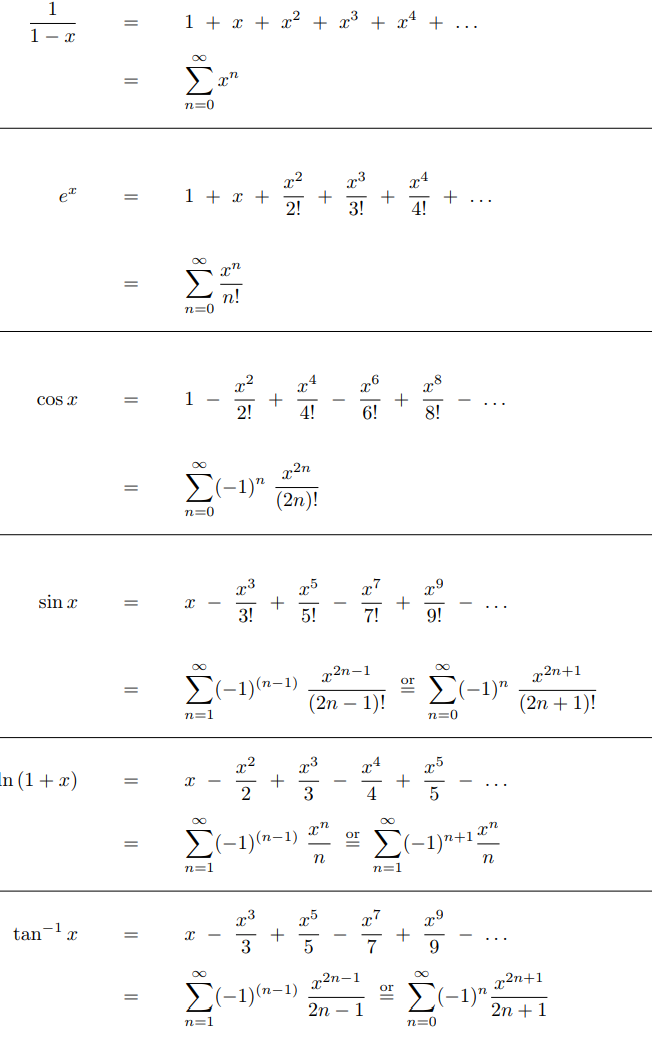
\includegraphics[width=0.7\linewidth]{common_taylor_series}



\section{Sequences}
\textbf{Convergent sequence:}A sequence $\{z_n\}$ is said to have a limit $z_0$ or converge to $z_0$ which we write as 
	
	$$\lim_{n\to\infty} z_n = z_0$$
	
	if for every $\epsilon > 0, \exists\ M \in  \mathbb{Z}$, such that:
	
	$$|z_n - z_0| < \epsilon,\ \forall n > M$$

\textbf{Cauchy Sequence:} a sequence $\{z_m\}$ of complex numbers is a Cauchy sequence if for every $\epsilon>0$, $\exists N \in \mathbb{Z}$ such that $|z_m - z_M| < \epsilon,\ \forall m, M>N$.

\textbf{Cauchy Criterion for Series Convergence} Let $s_m = \sum_{k=1}^{m}a_k$. The series $\sum_{k=1}^{\infty}a_k$ converges if and only if for every $\epsilon>0$, there exists $N \in \mathbb{Z}$ for $m, M>N$:

$$|s_M - s_m| = \left|\sum_{k=m+1}^{M}a_k\right| < \epsilon$$

Alternatively, letting $M = m+p$:

$$|s_{m+p} - s_m| = \left|\sum_{k=m+1}^{m+p}a_k\right| < \epsilon, \forall p = 1,2,3,..$$

This is the most general test for convergence of a series. 
\textbf{Radius of Convergence}:The power series $\sum_{m=0}^\infty a_m z^m$ has a radius of convergence $R = \frac{1}{A}$, where $A =\lim\sup_{m \to \infty } |a_m|^{1/m}$. If $A = \infty$, $R = 0$. Likewise, if $A=0$, $R = \infty$.

\begin{theorem}[Weirstrass M-test]
	Let $M_m$ be a sequence of real numbers. Suppose that $|f_m(z)| < M_m, \forall z \in E, m\in \mathbb{Z}^+$.  If $\sum_{m=1}^\infty M_m$ converges, then $\sum_{m=1}^\infty f_m(z)$ converges uniformly and absolutely on $E$. 
\end{theorem}
 
\textbf{Harmonic function}: Satisfies $\pdv{^2u}{x^2} + \pdv{^2u}{y^2} = 0$
\textbf{Analyticity}: Differentiable everywhere in neighborhood of point.
\textbf{Roots of Unity}: The $k$th root of unity is $\omega$ s.t. $\sum_{n=1}^{k} w^n =0$
\textbf{Entire Function} holomorphic/analytic all over 


\section{Branch Points and Branch Cuts}
NOTE: only have to say what it is. 
\begin{itemize}
	\item $z^p$, $p$ non integer has BP at 0, $\infty$.
	\item $\log z$ BP at 0, $\infty$
\end{itemize}

\begin{tabular}{|c|c|}
	\hline 
	Function & Branch Point \\ 
	\hline 
	$z^p$, non-integer p & $z = 0, \infty$ \\ 
	\hline 
	$log(z)$ &  $z = 0, \infty$\\ 
	\hline 
\end{tabular} 
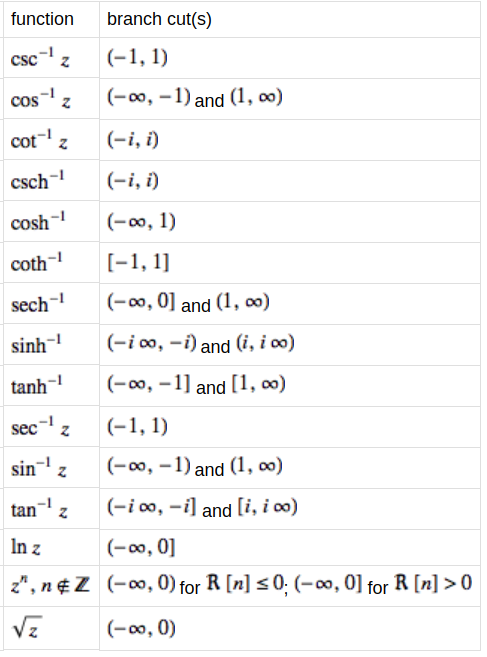
\includegraphics[width=0.7\linewidth]{branch_cuts}

\section{Singularities}
Isolated singularities
\begin{itemize}
	\item \textbf{Pole}: $f$ can be written as $g/(z-z_0)$
	\item \textbf{Removable}: $z_0$ is analytic in neighborhood and limit exists. Chuanpeng says this is not a singularity.
	\item \textbf{Essential} Neither, yet isolated. Ex. $f(z) = \frac{\sin z}{z}$.
\end{itemize}
Non-isolated singularities: each deleted neighborhood has a singularity. e.g. branch points, $2\frac{1}{\sin(1/z)}$

\section{Taylor/Maclaurin series expansion}
Maclaurin is just taylor about $z=0$.

\section{Laurent Series Expansions}
Two cases:
\begin{enumerate}
	\item $f$ analytic in circle around expansion point. Use Taylor Series Expansion.
	\item $f$ analytic in annulus. Then find Laurent series through something like change of variables to get series.
\end{enumerate}
\textbf{Gauss Mean Value}:
Suppose $f(z)$ is analytic in the closed disk $|z-z_0| \leq r$. Then:
$$f(z_0) = \frac{1}{2 \pi } \int_{0}^{2\pi} f(z_0 + r e^{i\theta} d\theta)$$

\textbf{Cauchy Integral Formula}
If $f$ analytic, $C$ simply connected and closed, $z_0 \in C$, then $f(z_0) = \frac{1}{2\pi i}\int_{C} \frac{f(z)}{z-z_0}dz$. Also $f^{(n)}(z_0) = \frac{n!}{2\pi i } \int_C \frac{f(z)}{(z-z_0)^{n+1}}dz$

\textbf{Cauchy Riemmann Equations} Necessary but NOT sufficient for differentiability at a point. Applied to neighborhood is sufficient for analyticity. Or if $u, v$ have continuous partials in domain $D$. 
Given $f(z) = u(x,y)+iv(x,y)$:
$$\frac{\partial u}{\partial x} = \frac{\partial v}{\partial y},\ \frac{\partial v}{\partial x} = -\frac{\partial u}{\partial y}$$
OR

$$f'(z) = \frac{\partial f}{\partial x} = -i \frac{\partial f}{\partial y}$$
OR 
Let $f=u+iv$ be differentiable with complex partials at $z=re^{i\theta}$. Then:
$$\pdv{u}{r} = \frac{1}{r} \pdv{v}{\theta},\ \pdv{v}{r} = -\frac{1}{r} \pdv{u}{\theta}$$


\textbf{Indented Path lemma}
Let $f$ have a simple pole at $a$ with a residue $\Res[f;a]$. Then given an upper half clockwise semi-circular contour around the pole $C_\epsilon$, the resulting contour is:

\begin{align}
\lim_{\epsilon\to0} \int_{C_\epsilon} f(z) dz = -\Res[f;a]\pi i
\end{align}

\textbf{Jordan's lemma}: If $C_R$ is the positive imaginary semicircular contour, the only singularities in $g(z)$ are poles, $a>0$, and $g(z) \to 0$ as $R \to \infty$, then 

$$\lim_{R \to \infty} \int_{C_R}e^{iaz}g(z) dz = 0$$

If you'd like to apply Jordan's lemma for $a<0$, try taking the semicircular contour that goes through the negative semicircular contour. Likewise, we can also say very carefully that Jordan's lemma.

\textbf{Residue theorem}: Suppose that $f(z)$ is analytic inside and on a simple closed contour $C$ except for isolated singularities at $z_1, z_2,..,z_n$ inside $C$. Let the residues at these points be $\alpha_1, \alpha_2,..,\alpha_n$ respectively. Then:
$\int_C f(z) dz = 2 \pi i \sum_{i=1}^n \alpha_i$

\textbf{Residue of simple pole of order k:} $a_{-1} = \frac{1}{(k-1)!} \lim_{z \to z_0} \dv{{}^{k-1}}{z^{k-1}} (z-z_0)^k f(z)$ 

\textbf{Sector integration: }take an arc-slice of a circle around a singularity (or two) and then go use residue theorem.

Maclaurin expansion of $f(z) = \log(z+1)$ valid for $|z|<1$. We know that $f'(z) = \frac{1}{1+z}$. This is just the same as a geometric series: $f'(z) = \sum_{n=0}^\infty (-1)^n z^n$

Hence:

\begin{align}
f(z) &= \log(1+z) \\ 
& = \int_{0}^z f'(\zeta) d\zeta + f(0) \\ 
& = \sum_{n=0}^\infty \int_{0}^z (-1)^n\zeta^n d\zeta + 0 \\ 
&  = \sum_{n=0}^\infty \frac{(-1)^n\zeta^{n+1}}{n+1}  
\end{align}
\section{Special Functions}
\textbf{Gamma function:} $\Gamma(z) = \int_0^\infty x^{z-1} e^{-x} dx$

The infinite form:
$\lim_{n\to\infty} \Gamma(z;n) := \int_{0}^{n} (1-\frac{t}{n})^n t^{z-1} dt = \Gamma(z) =  $
Integer: $n \in \mathbb{Z}^+$, $\Gamma(n) = (n+1)!$ 
Properties of Gamma function
\begin{itemize}
	\item $\Gamma(1) = 1$
	\item $\Gamma(z+1) = z \Gamma(z)$ 
	\item $\Gamma (z)={\frac {1}{z}}\prod _{n=1}^{\infty }{\frac {\left(1+{\frac {1}{n}}\right)^{z}}{1+{\frac {z}{n}}}}$
	\item $\Gamma (1-z)\Gamma (z)={\pi  \over \sin(\pi z)},\qquad z\not \in \mathbb{Z} $
	\item $\Gamma(\frac{1}{2}) = \sqrt{\pi }$
	\item $ \Gamma (z)={\frac {\Gamma (z+n+1)}{z(z+1)\cdots (z+n)}}$
	\item $\Gamma(\frac{1}{2} + z) \Gamma(\frac{1}{2} - z) = \frac{\pi}{\cos \pi z}$ 
	\item $\beta(p,q) = \frac{\Gamma(p)\Gamma(q)}{\Gamma(p+q)}$
	\item $(1+z)^\alpha = \sum_{n=0}^\infty \frac{\Gamma(\alpha+1)}{n!\Gamma(\alpha-n+1)}z^n$ (use the factorial identity)
	\item $\log \Gamma(z) = -\log z - \gamma z - \sum_{k=1}^\infty \left[\log(1+\frac{z}{k}) - \frac{z}{k}\right]$
	\item $\Res[\Gamma, -n] = \frac{(-1)^n}{n!}$
\end{itemize}

\textbf{Beta Function}: $ \mathrm{B} (x,y)=\int _{0}^{1}t^{x-1}(1-t)^{y-1}\,dt
= \frac{\Gamma(x)\Gamma(y)}{\Gamma(x+y)}$

\textbf{Psi Function:}$\Psi (z) = \frac{\Gamma'(z)}{\Gamma(z)} = \dv{z} \left(\log \Gamma(z)\right)$, with $\Psi(1) = -\gamma$, where $\gamma$ ie the Euler-Mascheroni Constant. 

\textbf{Riemann Zeta Function}: 
$\zeta(s) = \sum_{n=0}^{\infty} \frac{1}{(1+n)^\zeta}$
Relation to prime numbers
$\frac{1}{\zeta(s)} = \prod_{p} (1-\frac{1}{p^s}),\ p \in \text{Primes}$

\textbf{Bessel Equation Definitions}
1st kind: $J_\nu (z) = \left(\frac{z}{2}\right)^\nu \sum_{n=0}^{\infty} \frac{(-1)^n}{n! \Gamma(\nu+n+1)} \left(\frac{z}{2}\right)^{2n}$
$J_{-n}(x) = (-1)^nJ_n(x)$
$J_n(x) = \frac{1}{\pi} \int_0^\infty \cos(n\tau - x \sin\tau)$
$J_n(x) = \frac{1}{2\pi} \int_{-\pi}^{\pi} e^{i(x\sin\tau n\tau)} d\tau $

2nd Kind: $Y_{\alpha }(x)={\frac {J_{\alpha }(x)\cos(\alpha \pi )-J_{-\alpha }(x)}{\sin(\alpha \pi )}}$

\textbf{Legendre Polynomials}:
$P_n = \frac{1}{2^n n!} \dv{^n}{z^n} [(z^2-1)^n]$
$P_0(z) = 1,\ 
P_1(z) = z,\ 
P_2(z)= \frac{1}{2}(3z^2-1) 
$

\textbf{Generating Function}: $\phi(\zeta, z) = P_0(z) + \zeta P_1(z) + \zeta^2 P_2(z) + ...$


\section{Fourier Transform}
Fourier Transform:$F(\lambda) = \frac{1}{\sqrt{2\pi}} \int_{-\infty}^{\infty} e^{i \lambda \tau} f(\tau) d\tau$
Inverse Fourier Transform: 
$f(t) = \frac{1}{\sqrt{2\pi}} \int_{-\infty}^\infty F(\lambda) e^{-i\lambda \tau} d\lambda $
\subsection{Properties of the Fourier Transform}
For a function $f(t)$ with Fourier Transform $F(\lambda)$
\begin{itemize}
	\item $I.F.T.[f(t)] = F(-\lambda)$
	\item For constants $a,b$: $F.T.[af(t)+bg(t)] = a F.T.[f(t)] + b F.T.[g(t)] $
	\item $F.T.[f(t)g(t)] = F.T.[f(t)] * F.T.[g(t)]$  where $*$ is the convolution operator.
	\item $F.T.[f(t) * g(t)] = F.T.[f(t)] F.T.[g(t)]$
	\item $F.T.[\dv{^n}{t^n} f(t)] = (-i\lambda)^n F(\lambda)$
	\item $F.T.[\delta(t)] = \frac{1}{\sqrt{2\pi}}$
	\item $F.T.[1] = \frac{1}{\sqrt{2\pi}}\delta(-t) = \frac{1}{\sqrt{2\pi}}\delta(t)$
	\item $F.T.[f(t-t_0)] = \frac{1}{\sqrt{2\pi}}  \int_{-\infty}^\infty e^{i \lambda t} f(t-t_0) dt = \frac{1}{\sqrt{2\pi}}  \int_{-\infty}^\infty e^{i \lambda (t'+t_0)} f(t') dt' = e^{i \lambda t_0} F(\lambda)$
	\item $F.T.[\delta(x-\xi)\delta(y-\nu)\delta(z-\zeta)] = \left(\frac{1}{\sqrt(2 \pi)}\right)^3 e^{-(X\xi + Y\nu + Z \zeta)}$
\end{itemize}

F.T. of Gaussian:
$g(x) = \frac{1}{\sigma \sqrt{2 \pi}} e^{\frac{-x^2}{2\sigma^2}}, G(\omega) = e^{-\frac{\omega^2 \sigma^2}{2}}$

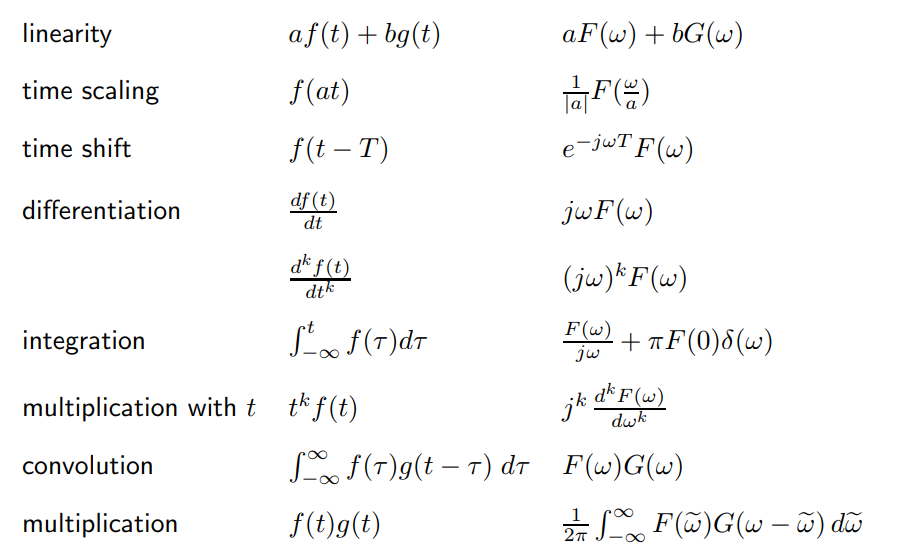
\includegraphics[width=0.7\linewidth]{common_fourier}

\textbf{Parseval's theorem for Fourier}:
$\int_{-\infty}^{\infty} |F(\lambda)|^2 d\lambda =  \int_{-\infty}^{\infty} |f(x)|^2dx $

This is analogous to \textbf{Parseval's identity for Fourier series:}

$\frac{1}{T} \int_{-T}^{T} f^2(t) dt = \frac{1}{2} a_0^2  + \sum_{n=1}^\infty (a_n^2 + b_n^2)$

\textbf{3D Fourier:}
$F(\mathbf{\lambda}) = \frac{1}{(2 \pi)^{3/2}} \iiint_{-\infty}^\infty e^{i \mathbf{\lambda x}} f(\mathbf{x}) dv_\mathbf{x}$
\textbf{Fourier Coefficients}: 

\textbf{Green's function}: Solution to $LG = \delta$ for linear differential operator $L$.
To find this for some ODE, set the forcing function to $\delta(x-\xi)$, then the solution $u$ is the green's function. 

$u_t - ku_xx = 0$ with $u(x,0) = \delta(x)$ has the kernel function:
$G(x,t) = \frac{1}{\sqrt{4 \pi k t}} \exp \left(-\frac{x^2}{4kt}\right)$,
For an n dimensional equation:
$U(x_1,,...x_n,t) = \frac{1}{\sqrt{(4 \pi k t)^n}} \exp \left(-\frac{\mathbf{x \cdot x}}{4kt}\right)$,
Then the forced solution is the convolution with the initial condition$u(x,0) = g(x)$
$u(x,t) = \int U(x-y, t) g(y) dy$

The Green's function $G(x,t;\xi)$ is the solution with $\delta(x-\xi)$:
$G(x,t;\xi) =  G(x- \xi,t) =\frac{1}{\sqrt{4 \pi k t}} \exp \left(-\frac{(x-\xi)^2}{4kt}\right)$,



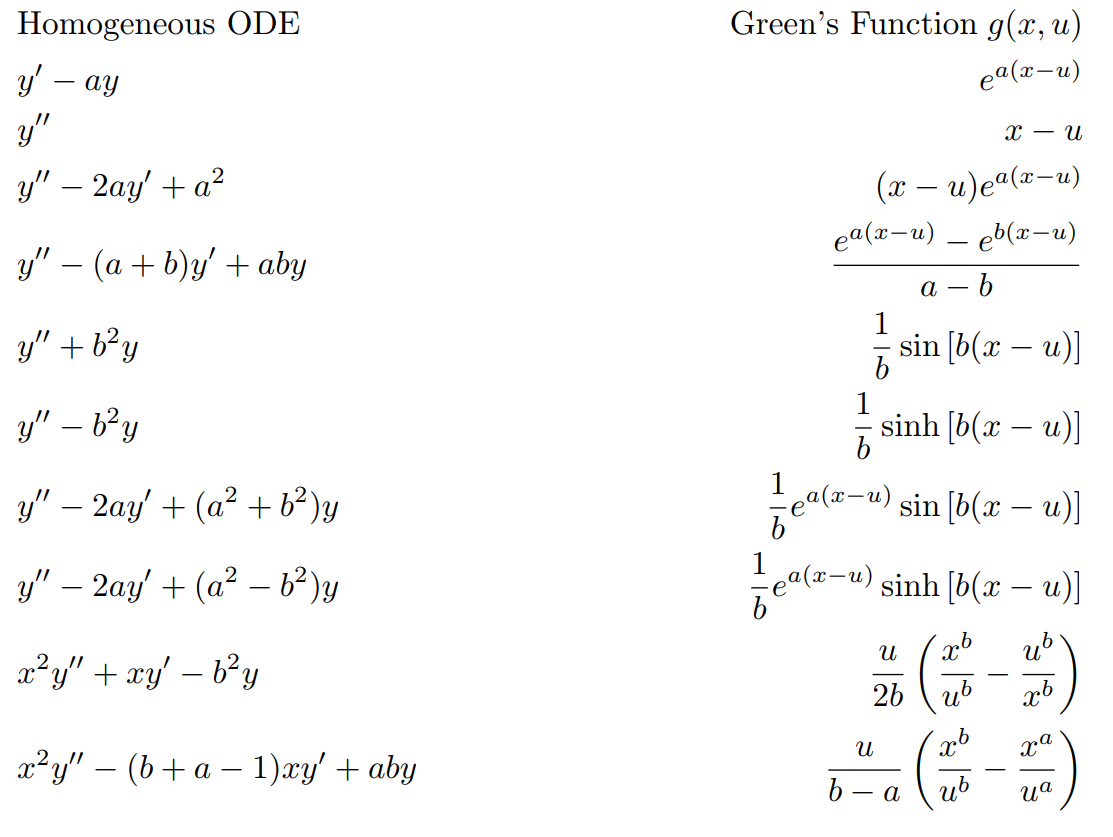
\includegraphics[width=0.7\linewidth]{green_common}



\subsection{Laplace Transform}
$F(s) = \int_{-\infty}^\infty f(t) e^{-st} dt$
Inverse L.T.:
$f(t) = \mathcal{L}^{-1}\{F(s)\}(t) = \frac{1}{2\pi i}\int_{\gamma - i \infty }^{\gamma + i \infty } e^{st} F(s) ds$

\textbf{Common Laplace Transforms:}

Gaussian: $\mathcal{L} [e^{-\pi x^2}] = \frac{1}{2} e^{\frac{\pi s^2}{4}} [\frac{1}{2} - \frac{1}{2} \erf{\frac{s\sqrt{\pi}}{2}}]$

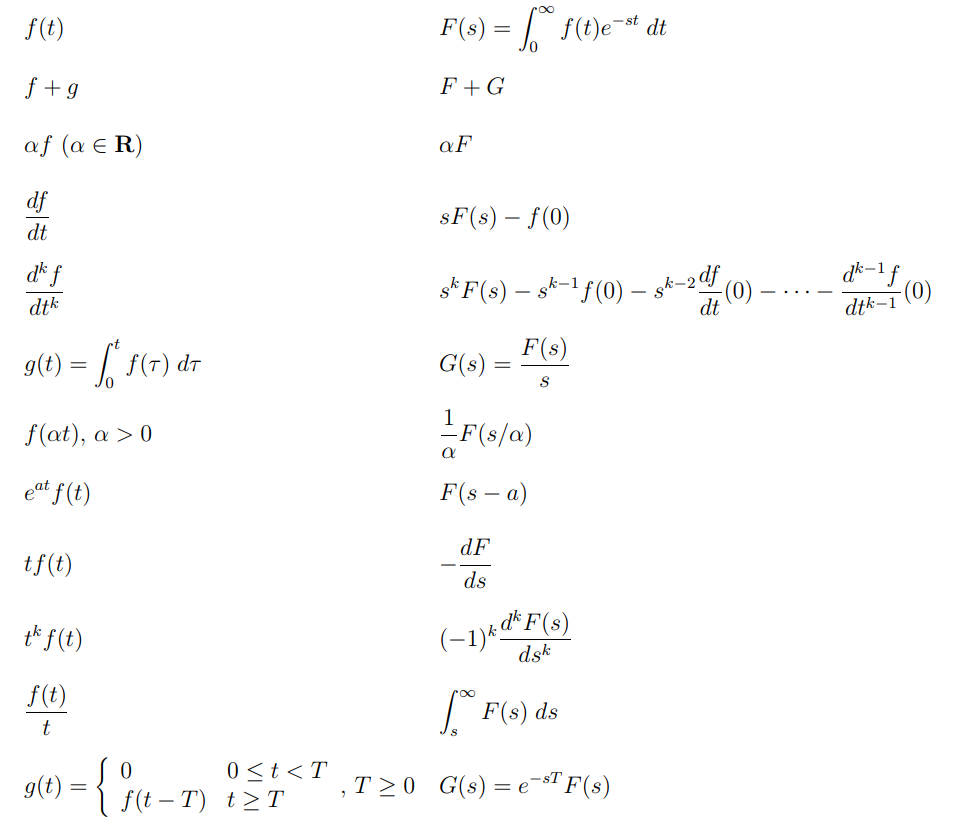
\includegraphics[width=1\linewidth]{general_laplace}
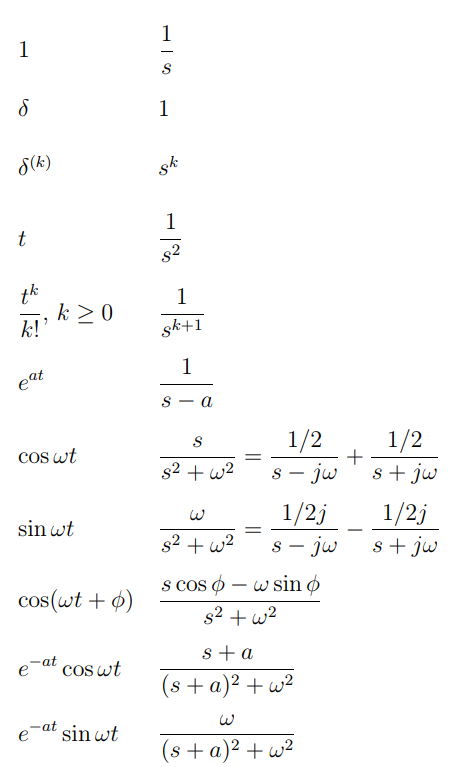
\includegraphics[width=0.7\linewidth]{specific_laplace}

\textbf{Multiplication and convolution of Laplace Transform:}
$f(t)g(t) = \frac{1}{2\pi i} \int_{\gamma - i \infty }^{\gamma+i\infty } F(x) G(s-x) dx$
$(f * g)(t) = \int_0^t f(\tau)g(t-\tau) d\tau = F(s)G(s)$

\subsection{Convolution}:
$f \conv g = \frac{1}{\sqrt{2 \pi}} \int_{-\infty}^{\infty} f(\xi) g(x - \xi) d\xi$

\textbf{Properties of $\delta$ function:}
\begin{itemize}
	\item $\delta(-t) = \delta(t)$ 
	\item $\delta(at) = \frac{1}{|a|}\delta(t)$
	\item $t\delta(t) = 0$
	\item $\delta(t^2 - a^2) = \frac{1}{2|a|}\left[\delta(t+a) + \delta(t-a)\right]$
	\item $\delta(t) = -t \delta ' (t) \ (I.B.P.)$
\end{itemize}

\subsection{Solving differential equations}
To solve $y''(x) + xy' ... = 0$, write out as series and solve:

$y(x) = \sum_{n=0}^{\infty}a_n x^n$
$y'(x) = \sum_{n=0}^{\infty}(n+1)a_{n+1} x^n = \sum_{n=1}^{\infty}(n)a_{n} x^{n-1}$
$y''(x) = \sum_{n=0}^{\infty}(n+1)(n+2)a_{n+2} x^n = \sum_{n=2}^{\infty} n(n-1) a_nx^n$

Substitute in and then we see that the sum $\sum C a_n + B a_{n+k} = 0$, then $ C a_n + B a_{n+k} = 0$ so then solve for $a_{n+k}$ in terms of $a_n$ to get a recursive equation. There is also usually an $a_0$ case or whatever, and you can go solve for the odd and even series or every $n=2k$ series or whatever. \\

How do we know when these infinite sums terminate? if it's $(a-1)...(a-2k-2)$ or something, then it terminates if $a$ is a positive odd integer, then maybe expand to say that it is about all integers. \\


\textbf{Laplacian Operator:} $\Delta f = \nabla\nabla f $, where $\nabla = (\dv{x_1},..., \dv{x_n})$.
Cartesian:
$ \Delta f={\frac {\partial ^{2}f}{\partial x^{2}}}+{\frac {\partial ^{2}f}{\partial y^{2}}}+{\frac {\partial ^{2}f}{\partial z^{2}}} $

Cylindrical:
$ \Delta f={\frac {1}{\rho }}{\frac {\partial }{\partial \rho }}\left(\rho {\frac {\partial f}{\partial \rho }}\right)+{\frac {1}{\rho ^{2}}}{\frac {\partial ^{2}f}{\partial \varphi ^{2}}}+{\frac {\partial ^{2}f}{\partial z^{2}}}$

Spherical:

$\begin{aligned}\Delta f&={\frac {1}{r^{2}}}{\frac {\partial }{\partial r}}\left(r^{2}{\frac {\partial f}{\partial r}}\right)+{\frac {1}{r^{2}\sin \theta }}{\frac {\partial }{\partial \theta }}\left(\sin \theta {\frac {\partial f}{\partial \theta }}\right)+{\frac {1}{r^{2}\sin ^{2}\theta }}{\frac {\partial ^{2}f}{\partial \varphi ^{2}}}\\&={\frac {1}{r}}{\frac {\partial ^{2}}{\partial r^{2}}}(rf)+{\frac {1}{r^{2}\sin \theta }}{\frac {\partial }{\partial \theta }}\left(\sin \theta {\frac {\partial f}{\partial \theta }}\right)+{\frac {1}{r^{2}\sin ^{2}\theta }}{\frac {\partial ^{2}f}{\partial \varphi ^{2}}}\end{aligned}$


$F.T.[\Delta f(x,y,z) + k^2 \dv{f}{t}] = -(X^2 + Y^2 + Z^2)F + k^2 F$ 
\section{ODE}
Solving IVP:
\begin{enumerate}
	\item Transform D.E. using initial conditions and laplace
	\item Solve for $Y(s)$
	\item IFT for $y(t)$.
\end{enumerate}

Also try $u(x,t) = X(x), T(t)$, then for $u_t, u_{xx}$ you can integrate separately.
\subsection{First order ODE}
$\dv{U}{t} = -k\lambda^2 U$
Then
$U(\lambda, t) = C(\lambda)e^{-k\lambda^2 t}$ 

\subsection{Second Order ODE}
Constant coefficient:$ay''(x) + by'(x) + cy(x) = f(x)$
$y(x) = e^{rx} \to ar^s + br + c = 0$
Cases:

Distinct, real roots: $r = r_{1,2}, y_h(x) = c_1 x^{r_1}  + c_2 x^{r_2}$\\
One real root: $y_h(x) = (c_1 + c_2 \ln |x| )x^r$\\
Complex roots: $r = \alpha + i \beta,$ $y_h(x) = (c_1 \cos ()\beta \ln |x|) + c_2 \sin (\beta \ln |x|))x^\alpha$\\
Further:
$-k^2U(\lambda, y) = \dv{^2}{y^2}U(\lambda,y)$
has solution:
$U(\lambda,y) = A(\lambda)e^{-|\lambda|y}$
Furthermore:
$y'' + \lambda y = 0$
\begin{itemize}
	\item $\lambda>0$: $y = a \cos (\sqrt{\lambda}x) + b \sin (\sqrt{\lambda}x) $
	\item $\lambda = 0$: $y = a + b x$
	\item $ \lambda < 0$: $y = a \cosh (\sqrt{-\lambda}x) + b \sinh (\sqrt{-\lambda}x) $
\end{itemize}

\end{multicols}
\end{document}


